\documentclass[border=3pt]{standalone}
% Preâmbulo compartilhado pelos diagramas TikZ da aula 5 de IHC (Processos de Design)
\usepackage[T1]{fontenc}
\usepackage[utf8]{inputenc}
\usepackage{lmodern}
\usepackage{amsmath}
\usepackage{xcolor}
\usepackage{tikz}
\usetikzlibrary{arrows.meta,angles,quotes,decorations.pathmorphing,calc,
                positioning,shapes.geometric,shapes.misc,backgrounds,fit,
                math}

% Paleta (mesma dos SVGs originais)
% Paleta da disciplina de IHC: acento roxo (#755099), da capa do livro.
% (o nome "dblue" é mantido para não alterar todos os diagramas)
\definecolor{dblue}{HTML}{755099}
\definecolor{dorange}{HTML}{B3541E}
\definecolor{dgreen}{HTML}{4A7C59}
\definecolor{dred}{HTML}{9C4B4B}
\definecolor{dcream}{HTML}{F4F1EA}
\definecolor{dshade}{HTML}{DDD7C9}

% Função gaussiana (não normalizada por padrão de escala visual)
\pgfmathdeclarefunction{gauss}{3}{%
  \pgfmathparse{1/(#3*sqrt(2*pi))*exp(-((#1-#2)^2)/(2*#3^2))}%
}

% Estilos comuns (prefixo d... para não colidir com chaves internas do pgf)
\tikzset{
  >={Stealth[length=2mm]},
  dguide/.style={gray!55, dashed, line width=0.4pt},
  daxis/.style={gray!60, line width=0.7pt, ->},
  dbody/.style={fill=black!3, draw=black!80, line width=1pt},
  dacc/.style={draw=dblue, line width=1pt},
  dlbl/.style={black!55, font=\small},
  dsub/.style={black!45, font=\footnotesize},
  dstate/.style={circle, draw=black!80, fill=dcream, line width=1pt,
                 minimum size=17mm, font=\large, inner sep=1pt},
  dobs/.style={circle, draw=black!80, fill=dshade, line width=1pt,
               minimum size=14mm, font=\large, inner sep=1pt},
  dbox/.style={rounded corners=2pt, draw=black!80, fill=dcream, line width=1pt,
               align=center, inner sep=6pt},
  dop/.style={circle, draw=black!80, fill=white, line width=1pt,
              minimum size=6mm, inner sep=0pt, font=\small},
  dtrans/.style={->, dblue, line width=1pt},
  dmeas/.style={->, dorange, line width=1pt},
  dcurve/.style={line width=1pt, dblue},
  dcurveb/.style={line width=1.4pt, dorange},
}

\begin{document}
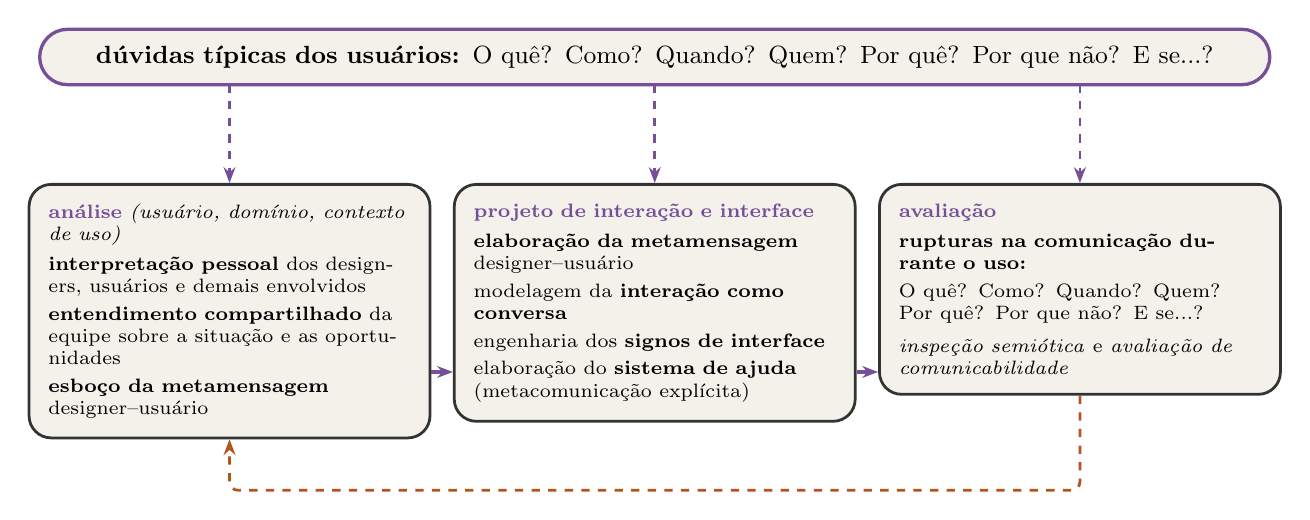
\begin{tikzpicture}[x=1cm,y=1cm,
   col/.style={dbox, rounded corners=8pt, text width=4.6cm, align=left, font=\scriptsize, inner sep=7pt, anchor=north}]

  \node[dbox, rounded corners=10pt, text width=15.2cm, font=\small, draw=dblue, line width=1.2pt] (top) at (7.0,0) {\textbf{dúvidas típicas dos usuários:} O quê? Como? Quando? Quem? Por quê? Por que não? E se...?};

  \node[col] (c1) at (1.6,-1.6) {\textbf{\textcolor{dblue}{análise}} \textit{(usuário, domínio, contexto de uso)}\\[3pt]
     \textbf{interpretação pessoal} dos designers, usuários e demais envolvidos\\[2pt]
     \textbf{entendimento compartilhado} da equipe sobre a situação e as oportunidades\\[2pt]
     \textbf{esboço da metamensagem} designer--usuário};
  \node[col] (c2) at (7.0,-1.6) {\textbf{\textcolor{dblue}{projeto de interação e interface}}\\[3pt]
     \textbf{elaboração da metamensagem} designer--usuário\\[2pt]
     modelagem da \textbf{interação como conversa}\\[2pt]
     engenharia dos \textbf{signos de interface}\\[2pt]
     elaboração do \textbf{sistema de ajuda} (metacomunicação explícita)};
  \node[col] (c3) at (12.4,-1.6) {\textbf{\textcolor{dblue}{avaliação}}\\[3pt]
     \textbf{rupturas na comunicação durante o uso:}\\[2pt]
     O quê? Como? Quando? Quem? Por quê? Por que não? E se...?\\[4pt]
     \textit{inspeção semiótica} e \textit{avaliação de comunicabilidade}};

  \foreach \x in {1.6,7.0,12.4} { \draw[dtrans, dashed] (\x,-0.35) -- (\x,-1.6); }
  \draw[dtrans, line width=1.3pt] (c1.east |- 1.6,-4.0) -- (c2.west |- 1.6,-4.0);
  \draw[dtrans, line width=1.3pt] (c2.east |- 1.6,-4.0) -- (c3.west |- 1.6,-4.0);
  \draw[dmeas, dashed, rounded corners=3pt] (c3.south) -- ++(0,-1.2) -| (c1.south);


\end{tikzpicture}
\end{document}
